\documentclass[UTF8,oneside,openany]{ctexbook}
\usepackage{braket}
\usepackage{graphicx}
\usepackage{geometry}
\geometry{a4paper,left=2cm,right=2cm,top=2cm,bottom=2cm}
\usepackage[nottoc]{tocbibind}
\usepackage{amsmath}
\usepackage{amssymb}
\usepackage{cases}
\usepackage{balance}
\DeclareMathOperator\dif{d\!}
\usepackage{mathtools}
\usepackage{xcolor}
\usepackage[colorlinks=true,citecolor=blue,urlcolor=black]{hyperref}
\hypersetup{colorlinks}
\newcommand\innp[2]{\langle#1|#2\rangle}
\newcommand\aver[1]{\langle#1\rangle}
\newcommand\digg[1]{{\hat{#1}}^{\dagger}}
\newcommand\kb{k_{\text{B}}}

\usepackage{titlesec}
\usepackage{titletoc}
\usepackage[toc]{multitoc}
\titlecontents{chapter}
[6em]
{\vspace{3mm}\heiti}
{\contentslabel{4.5em}}
{}
{\titlerule*[0.5pc]{$\cdot$}\small\contentspage}
\titlecontents{section}
[4em]
{\small}
{\contentslabel{2.5em}}
{}
{\titlerule*[0.5pc]{$\cdot$}\contentspage}
\titlecontents{subsection}
[7em]
{\small}
{\contentslabel{3.3em}}
{}
{\titlerule*[0.5pc]{$\cdot$}\contentspage}

\title{\heiti 统计力学}
\author{\empty}
\date{\empty}
\pagestyle{plain}

\begin{document}

\maketitle
\hypersetup{linkcolor=black}
\tableofcontents
\thispagestyle{empty}
\newpage
\setcounter{page}{1}
\hypersetup{linkcolor=blue}

\chapter{微正则系综}
\section{微正则系综}
考虑由$N$个粒子组成的系统,其微观状态取决于所有粒子的运动状态,即,由系统中所有粒子的广义动量和广义坐标
\begin{equation}
p_1,\cdots,p_{3N};q_1,\cdots,q_{3N}
\end{equation}
决定。引入由这$3N$个广义动量和$3N$个广义坐标为直角坐标的$6N$维相空间,称之为$\Gamma$空间,则系统在某一时刻的运动状态就可用相空间中的一点来表示,该点称为系统运动状态的代表点。系统状态的变化对应着代表点的运动,满足哈密顿正则方程
\begin{equation}
\dot{p_i}=-\frac{\partial H}{\partial q_i}\qquad
\dot{q_i}=\frac{\partial H}{\partial p_i}
\end{equation}
任何物理测量总是在一个宏观短、微观长的时间$T$内进行的,在这段时间内,系统的微观状态已经千变万化,因此测得的宏观量应是在这段观测时间内对观测量$\mathcal{O}(t)$的时间平均
\begin{equation}\label{ot}
\aver{\mathcal{O}}=\aver{\mathcal{O}}_t=\frac1T\int_{0}^T\mathcal{O}(t)\dif t
\end{equation}
对于平衡态系统,宏观量不随时间变化。只要物理测量是在宏观短、微观长的时间内进行,那么测量时间的长短对宏观量就不再重要,因此可以认为在这段时间内系统已经遍历了一切可能的微观状态(此即各态历经假设,或称遍历假设),于是测得的宏观量应是对一切可能的微观状态的统计平均,即系综平均
\begin{equation}\label{oe}
\aver{\mathcal{O}}=\aver{\mathcal{O}}_e=\int\mathcal{O}(\pmb{p},\pmb{q})\rho (\pmb{p},\pmb{q})\dif\Omega'
\end{equation}
其中
\begin{equation}
\dif\Omega'=\frac{\dif\Omega}{h^{3N}N!}=\frac{\dif\pmb{p}\dif\pmb{q}}{h^{3N}N!}=\frac{\dif p_1\cdots\dif p_{3N}\dif q_1\cdots\dif q_{3N}}{h^{3N}N!}
\end{equation}
式中$\rho(\pmb{p},\pmb{q})$是$\Gamma$空间中的代表点数密度分布函数。$h^{3N}$为相格大小\footnote{相格问题此处不想深究,感兴趣的可以参见\cite{h}及相关专著},$N!$是考虑粒子全同性带来的吉布斯修正因子。结合式\ref{ot}和式\ref{oe}我们就得到
\begin{equation}
\aver{\mathcal{O}}=\aver{\mathcal{O}}_t=\aver{\mathcal{O}}_e
\end{equation}
于是我们的任务就变成了确定$\rho(\pmb{p},\pmb{q})$。考虑孤立系统的情况,孤立系统能量守恒,所以系统的代表点应在相空间中的某个等能面上运动。刘维尔定理告诉我们$\dif\rho/\dif t=0$,即沿着由哈密顿正则方程确定的相轨道,$\rho$为常数,各态历经假设\footnote{事实上,从数学上可以证明严格的各态历经并不成立,但是因为实际的宏观孤立系统并非绝对的孤立,总是存在着外界对系统的微弱干扰,正是由于这种干扰,使代表点从一条相轨道转移到另一条相轨道,在足够长的时间内,代表点将经历许许多多相轨道,从而跑遍了能量曲面$E\sim E+\Delta E$的所有点,从而在物理上保证了各态历经(也正因此,许多教材的写法是$E\le H\le E+\Delta E$时$\rho=1/W$)。这一观点的正确性可由平衡态统计理论的全部推论和实验符合而得到充分肯定。当然,例外也是有的,例如多体局域化(many body localization)就不满足各态历经,此时平衡态统计力学已不再适用,我们需要寻求一个更普适的理论}说明在测量时间内系统已经经历了等能面上的所有微观状态,于是我们得到在整个等能面上$\rho$为常数的结论(此即等概率原理),即
\begin{equation}
\rho=\begin{cases}{}
1/W\qquad H=E\\
0\qquad\ \ \ \ \  H\neq E
\end{cases}
\end{equation}
$W$为等能面上的总微观状态数,我们有
\begin{equation}
W=\int\limits_{H=E}\dif\Omega'=\frac{1}{h^{3N}N!}\int\limits_{H=E}\dif\Omega
\end{equation}
我们将会看到整个平衡态统计力学可以由等概率原理导出。接下来我们通过几个例子来看看微正则系综给我们带来了什么。
\section{平衡条件与热力学量}
本节将讨论如何由微正则系综得到热力学量。考虑一个孤立系统$S$,它由两个只有微弱相互作用的系统$S_1$和$S_2$组成,$S_1$和$S_2$之间不仅可以交换能量,还可以交换粒子和改变体积,由于整个系统是孤立系,我们有
\begin{align}\label{ec}
E&=E_1+E_2\notag\\
N&=N_1+N_2\notag\\
V&=V_1+V_2
\end{align}
且总的微观状态数应为两个系统微观状态数的乘积,即
\begin{equation}
W(E,N,V)=W_1(E_1,N_1,V_1)W_1(E_2,N_2,V_2)
\end{equation}
对上式取对数得到
\begin{equation}
\ln W(E,N,V)=\ln W_1(E_1,N_1,V_1)+\ln W_2(E_2,N_2,V_2)
\end{equation}
由等概率原理我们知道,热力学平衡态必然是使$W$取极大值的宏观态,则
\begin{equation}
\delta\ln W=\biggl[\frac{\partial\ln W_1}{\partial E_1}-\frac{\partial\ln W_2}{\partial E_2}\biggr]\delta E_1+\biggl[\frac{\partial\ln W_1}{\partial N_1}-\frac{\partial\ln W_2}{\partial N_2}\biggr]\delta N_1+\biggl[\frac{\partial\ln W_1}{\partial V_1}-\frac{\partial\ln W_2}{\partial V_2}\biggr]\delta V_1=0
\end{equation}
上式用到了可由式\ref{ec}导出的$\partial E_2/\partial E_1=\partial N_2/\partial N_1=\partial V_2/\partial V_1=-1$。于是我们得到平衡条件
\begin{align}\label{ph1}
\frac{\partial\ln W_1}{\partial E_1}&=\frac{\partial\ln W_2}{\partial E_2}\notag\\
\frac{\partial\ln W_1}{\partial N_1}&=\frac{\partial\ln W_2}{\partial N_2}\notag\\
\frac{\partial\ln W_1}{\partial V_1}&=\frac{\partial\ln W_2}{\partial V_2}
\end{align}
令
\begin{align}\label{beta}
\beta&=\biggl(\frac{\partial\ln W}{\partial E}\biggr)_{N,V}\notag\\
\alpha&=\biggl(\frac{\partial\ln W}{\partial N}\biggr)_{V,E}\notag\\
\gamma&=\biggl(\frac{\partial\ln W}{\partial V}\biggr)_{N,E}
\end{align}
则式\ref{ph1}表示两系统$S_1$和$S_2$达到平衡的条件是
\begin{equation}\label{ph}
\beta_1=\beta_2\qquad\alpha_1=\alpha_2\qquad\gamma_1=\gamma_2
\end{equation}
热力学第零定律告诉我们,两系统达到热平衡的条件是温度相等,因此$\beta$与温度具有相同的作用。将玻尔兹曼关系\footnote{理论上来说,既然我们有了微正则系综,那么玻尔兹曼关系也应由此导出。此处为了简便起见,直接代入热力学中的玻尔兹曼关系。后面推导正则与巨正则系综中的熵也是直接代入热力学中的玻尔兹曼关系,不再赘述。}$S=\kb\ln W$以及热力学公式$\frac{1}{T}=(\frac{\partial S}{\partial E})_{N,V}$代入\ref{beta}第一式,我们有
\begin{equation}
\beta=\frac{1}{\kb T}
\end{equation}
$\ln W$的全微分为
\begin{equation}
\dif\ln W=\beta\dif E+\alpha\dif N+\gamma\dif V
\end{equation}
与开放系的热力学基本微分方程
\begin{equation}
\dif S=\frac1T\dif U+\frac{p}{T}\dif V-\frac{\mu}{T}\dif N
\end{equation}
比较可得
\begin{equation}\label{mup}
\alpha=-\frac{\mu}{\kb T}\qquad\gamma=\frac{p}{\kb T}
\end{equation}
因此,式\ref{ph}表示系统达到热力学平衡态时须满足的条件是
\begin{equation}
T_1=T_2\qquad p_1=p_2\qquad\mu_1=\mu_2
\end{equation}
上式分别为系统达到热力学平衡态时须满足的热平衡条件、力学平衡条件和相平衡条件。特别地,对于粒子数不守恒的系统,例如后面在实际应用中提到的声子和光子系统,不再有\ref{ec}第二式,也就不再有$\delta N_1=-\delta N_2$,此时$\delta N_1$和$\delta N_2$是独立变量可以自由变化,但为了满足$\delta\ln W=0$,因此我们有$\mu_1=\mu_2=0$,即粒子数不守恒的系统化学势$\mu=0$。至此我们由微正则系综得到了系统的熵、压强、化学势等热力学量,接下来我们将其应用到具体系统中。
\section{单原子理想气体}\label{ideal}
先来考查一下单原子理想气体,其哈密顿量为
\begin{equation}
H=\sum_{i=1}^{3N}\frac{p_i^2}{2m}
\end{equation}
直接计算等能面上的状态数较为复杂,简便方法是先计算等能面上及以内的所有状态数$\Sigma(E)$,然后对其微分就得到我们想要的$W(E)$
\begin{align}
\Sigma(E)&=\frac{1}{h^{3N}N!}\int\limits_{H\le E}\dif\Omega\notag\\
&=\frac{V^N}{h^{3N}N!}\int\limits_{\sum_{i=1}^{3N}p_i^2\le 2mE}\dif\pmb{p}\notag\\
\stackrel{\text{令$p_i=\sqrt{2mE}x_i$}}{=}&\frac{V^N}{h^{3N}N!}(2mE)^{3N/2}\int\limits_{\sum_{i=1}^{3N}x_i^2\le 1}\dif\pmb{x}\notag\\
&=\frac{V^N}{h^{3N}N!}(2mE)^{3N/2}K
\end{align}
其中$K$为$3N$维单位球体积,其计算结果为(见附录\ref{vo})
\begin{equation}
K=\int\limits_{\sum_{i=1}^{3N}x_i^2\le 1}\dif\pmb{x}=\frac{\pi^{3N/2}}{\Gamma(\frac{3N}{2}+1)}
\end{equation}
所以
\begin{equation}
\Sigma(E)=\frac{1}{N!}\biggl(\frac{V}{h^3}\biggr)^N\frac{(2\pi mE)^{3N/2}}{\Gamma(\frac{3N}{2}+1)}
\end{equation}
所以
\begin{equation}\label{lixiang}
W(E)=\frac{\partial\Sigma(E)}{\partial E}=\frac{3N}{2}\frac{1}{N!}\biggl(\frac{V}{h^3}\biggr)^N\frac{(2\pi mE)^{3N/2}}{\Gamma(\frac{3N}{2}+1)}\frac1E
\end{equation}
则
\begin{equation}
\ln W=N\ln\biggl[\frac{V}{Nh^3}\biggl(\frac{4\pi mE}{3N}\biggr)^{3/2}\biggr]+\frac52 N+\ln\frac{3N}{2E}
\end{equation}
上式在计算中运用了$\Gamma$函数的性质$\Gamma(N+1)=N!$以及斯特林近似公式$\ln N!=N\ln N-N$。最后一项与粒子的平均能量$\varepsilon=E/N$有关,当$N$很大时与前两项相比可略去。由式\ref{mup}可得气体压强为
\begin{equation}
p=\kb T\gamma=\kb T\biggl(\frac{\partial\ln W}{\partial V}\biggr)_{N,E}=\frac{N\kb T}{V}
\end{equation}
又
\begin{equation}
\frac{1}{T}=\biggl(\frac{\partial S}{\partial E}\biggr)_V=\kb\biggl(\frac{\partial\ln W}{\partial E}\biggr)_V=\frac{3N\kb}{2E}
\end{equation}
即
\begin{equation}
E=\frac32 N\kb T
\end{equation}
所以单原子理想气体的熵为
\begin{equation}
S=\kb\ln W=N\kb\ln\biggl[\frac{V}{N}\biggl(\frac{2\pi m}{\beta h^2}\biggr)^{3/2}\biggr]+\frac52 N\kb
\end{equation}
上述与我们已知的结论都是一致的。
\section{二能级系统}
考虑一个二能级系统,设基态能量为零,激发态能量为$\varepsilon$,激发态粒子数为$N_1$,则总的微观状态数为在$N$个粒子中挑选$N_1$个处在激发态的组合数,即
\begin{equation}
W=C_{N}^{N_1}=\frac{N!}{N_1!(N-N_1)!}
\end{equation}
系统的熵为
\begin{align}
S=\kb\ln W&=\kb\ln\frac{N!}{N_1!(N-N_1)!}\notag\\
&=-N\kb\biggl[\frac{N_1}{N}\ln\frac{N_1}{N}+\frac{N-N_1}{N}\ln\frac{N-N_1}{N}\biggr]\notag\\
&=-N\kb\biggl[\biggl(\frac{E}{N\varepsilon}\biggr)\ln\biggl(\frac{E}{N\varepsilon}\biggr)+\biggl(1-\frac{E}{N\varepsilon}\biggr)\ln\biggl(1-\frac{E}{N\varepsilon}\biggr)\biggr]
\end{align}
上式第二行运用了斯特林近似。于是我们有
\begin{equation}
\frac{1}{T}=\frac{\partial S}{\partial E}=-\frac{\kb}{\varepsilon}\ln\biggl(\frac{E}{N\varepsilon-E}\biggr)
\end{equation}
由此可得
\begin{equation}
E(T)=\frac{N\varepsilon}{\exp(\frac{\varepsilon}{\kb T})+1}
\end{equation}
粒子处在激发态的概率为
\begin{equation}
P_1=\frac{N_1}{N}=\frac{E}{N\varepsilon}=\frac{1}{\exp(\frac{\varepsilon}{\kb T})+1}
\end{equation}
即绝对零度时粒子全部处在基态,随着温度升高,粒子被不断地激发上去,这是非常自然的。
\chapter{正则系综}
\section{正则系综}
在实际应用中用微正则系综求平衡系统的热力学量往往不是很方便,即使对于像单原子理想气体这样简单的系统,系统微观状态数的计算也颇为复杂,而且孤立系比较特殊不具一般性。本章将讨论在实际应用中更普遍,在计算上也更简单的正则系综。

考虑一个与热源有热交换的封闭系统,令系统$S$和热源$R$组成一个复合的孤立系,由于外界的热源很大,当系统和源达到平衡时,系统具有与源相同的温度,因此这种系统是具有确定的体积$V$,温度$T$和粒子数$N$的封闭系统,由这种系统集合组成的系综是正则系综。如图所示
\begin{figure}[ht]
	\centering
	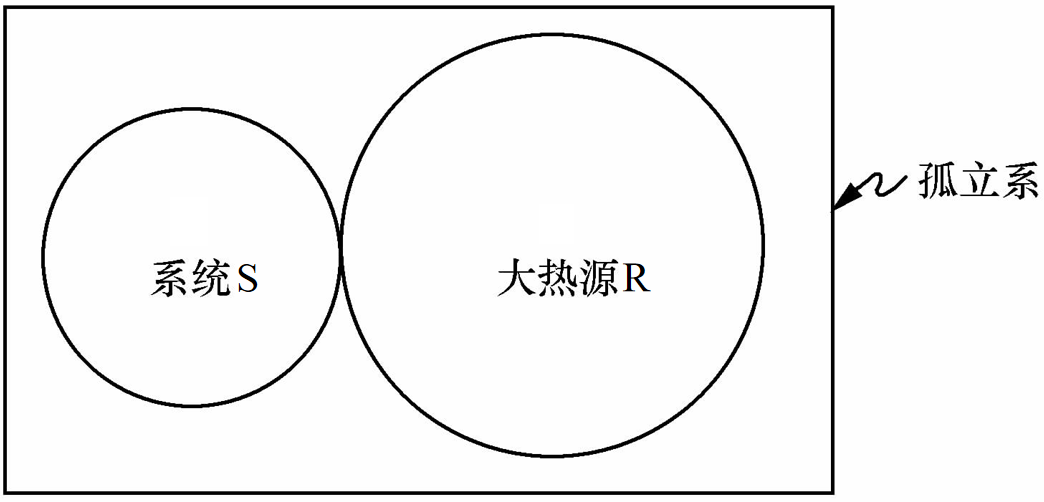
\includegraphics[scale=0.2]{ce.png}
	\caption{系统$S$和热源$R$组成一个复合的孤立系。}
\end{figure}

假设系统与热源之间的相互作用很弱,可以略去,则孤立系的能量为
\begin{equation}
E=E_s+E_r=const.
\end{equation}
当系统处于能量为$E_s$的微观状态$s$时,热源可处于能量为$E-E_s$的$W_r(E-E_s)$个微观状态中的任何一个。若孤立系的总微观状态数为$W$,根据等概率原理其处于任一可能状态的概率均为$\rho=1/W$。在孤立系的$W$个可能微观态中,有$W_r(E-E_s)$个对应着系统处于$s$态,因此系统处于$s$态的概率为
\begin{equation}\label{rs}
\rho_s=\frac{W_r(E-E_s)}{W}
\end{equation}
由式\ref{lixiang}可知微观状态数$W$随能量$E$变化非常剧烈,直接做泰勒展开其收敛必然很慢,为此讨论变化较为缓慢的对数函数$\ln W$。将$\ln W_r(E-E_s)$整体视作$\ln W_r(x)$在$x=E$处展开并忽略二次以上的小量,得到
\begin{equation}
\ln W_r(E-E_s)=\ln W_r(E)-E_s\biggl(\frac{\partial\ln W_r}{\partial E_r}\biggr)=\ln W_r(E)-\beta E_s
\end{equation}
将上式代入式\ref{rs},合并与$E_s$无关的因子可得
\begin{equation}\label{ps}
\rho_s=\frac1Z e^{-\beta E_s}
\end{equation}
$Z$称为系统的配分函数,其值由概率的归一化条件确定
\begin{equation}
Z=\sum_{s}e^{-\beta E_s}
\end{equation}
上式是对状态求和,如果我们有系统的能谱,则可以改写成对能级求和。系统处于第$\ell$个能级的概率为(设第$\ell$个能级的简并度为$g_{\ell}$)
\begin{equation}
\rho_{\ell}=\frac{g_{\ell}}{Z}e^{-\beta E_{\ell}}
\end{equation}
系综的配分函数为
\begin{equation}
Z=\sum_{\ell}g_{\ell}e^{-\beta E_{\ell}}
\end{equation}
当能级准连续(能级间隔$\Delta E_{\ell}\ll\kb T$)时须将求和换成积分,此时配分函数为
\begin{equation}
Z=\frac{1}{h^{3N}N!}\int e^{-\beta E(\pmb{p},\pmb{q})}\dif\Omega
\end{equation}
\section{配分函数与热力学量}
与微正则系综一样,我们可以由正则系综导出系统的热力学量,本节讨论如何由配分函数导出热力学量。热力学量$\mathcal{O}$的统计平均值为
\begin{equation}
\aver{\mathcal{O}}=\frac1Z\sum_{s}\mathcal{O}_se^{-\beta E_s}=\frac1Z\sum_{\ell}\mathcal{O}_{\ell}g_{\ell}e^{-\beta E_{\ell}}
\end{equation}
能级准连续时上式变为
\begin{equation}
\aver{\mathcal{O}}=\frac{1}{h^{3N}N!}\frac1Z\int\mathcal{O}(\pmb{p},\pmb{q})e^{-\beta E(\pmb{p},\pmb{q})}\dif\Omega
\end{equation}
系统的平均能量为
\begin{equation}\label{ae}
\aver{E}=\frac1Z\sum_{s}E_se^{-\beta E_s}=\frac1Z\biggl(-\frac{\partial}{\partial\beta}\biggr)\sum_{s}e^{-\beta E_s}=-\frac{\partial\ln Z}{\partial\beta}
\end{equation}
外界对系统的广义力$Y_i$是微观量$\frac{\partial E_s}{\partial y_i}$的统计平均值
\begin{equation}
\aver{Y_i}=\frac1Z\sum_{s}\frac{\partial E_s}{\partial y_i}e^{-\beta E_s}=\frac1Z\biggl(-\frac{1}{\beta}\frac{\partial}{\partial y_i}\biggr)\sum_{s}e^{-\beta E_s}=-\frac{1}{\beta}\frac{\partial\ln Z}{\partial y_i}
\end{equation}
若取$y_i=V$,则对应的广义力为$-p$,因此压强为
\begin{equation}\label{yq}
p=\frac{1}{\beta}\frac{\partial\ln Z}{\partial V}
\end{equation}
下面我们用正则分布导出熵的表达式,为此考虑
\begin{equation}
\beta(\dif U-Y\dif y)=-\beta\dif\biggl(\frac{\partial\ln Z}{\partial\beta}\biggr)+\frac{\partial\ln Z}{\partial y}\dif y
\end{equation}
$\ln Z$的全微分为
\begin{equation}
\dif\ln Z=\frac{\partial\ln Z}{\partial\beta}\dif\beta+\frac{\partial\ln Z}{\partial y}\dif y
\end{equation}
代入上式得
\begin{equation}
\beta(\dif U-Y\dif y)=\dif\biggl(\ln Z-\beta\frac{\partial\ln Z}{\partial\beta}\biggr)
\end{equation}
与封闭系的热力学基本微分方程
\begin{equation}
\frac1T(\dif U-Y\dif y)=\dif S
\end{equation}
比较可得
\begin{equation}
\dif S=\kb\biggl(\ln Z-\beta\frac{\partial\ln Z}{\partial\beta}\biggr)
\end{equation}
对上式积分并取积分常数为零可得
\begin{equation}\label{S}
S=\kb\biggl(\ln Z-\beta\frac{\partial\ln Z}{\partial\beta}\biggr)=\kb(\ln Z+\beta\aver{E})
\end{equation}
至此,我们从正则系综得到了系统的平均能量$\aver{E}$,广义力$Y_i$和熵$S$,系统的所有其他热力学量都可由这些量得到。

最后来看看正则系综的能量涨落,由式\ref{ae}对$\beta$求偏导得到
\begin{equation}
\frac{\partial\aver{E}}{\partial\beta}=-\frac1Z\sum_{s}E_s^2e^{-\beta E_s}-\frac{1}{Z^2}\frac{\partial Z}{\partial\beta}\sum_{s}E_se^{-\beta E_s}=-\aver{E^2}+\aver{E}^2
\end{equation}
因此能量涨落为
\begin{equation}\label{ezl}
\sigma_E=\aver{E^2}-\aver{E}^2=-\frac{\partial\aver{E}}{\partial\beta}=\kb T^2\biggl(\frac{\partial\aver{E}}{\partial T}\biggr)_{N,V}=\kb T^2C_V
\end{equation}
所以其相对涨落为
\begin{equation}\label{rezl}
\frac{\sigma_E}{\aver{E}^2}=\frac{\kb T^2C_V}{\aver{E}^2}
\end{equation}
\leftline{\heiti 单原子理想气体}
接下来我们用正则系综处理单原子理想气体,其哈密顿量已经在\ref{ideal}节给出,现在直接计算其配分函数
\begin{align}
Z&=\frac{1}{h^{3N}N!}\int e^{-\beta\sum_{i=1}^{3N}\frac{p_i^2}{2m}}\dif\Omega\notag\\
&=\frac{V^N}{h^{3N}N!}\int e^{-\beta\sum_{i=1}^{3N}\frac{p_i^2}{2m}}\dif p_1\cdots\dif p_{3N}\notag\\
&=\frac{V^N}{h^{3N}N!}\biggl(\int e^{-\beta\frac{p^2}{2m}}\dif p\biggr)^{3N}\notag\\
&=\frac{V^N}{h^{3N}N!}\bigg(\frac{2\pi m}{\beta}\bigg)^{\frac{3N}{2}}
\end{align}
由式\ref{ae},\ref{yq}和\ref{S}得到单原子理想气体的内能、压强和熵分别为
\begin{gather}
\aver{E}=-\frac{\partial\ln Z}{\partial\beta}=\frac32 N\kb T\notag\\
p=\frac{1}{\beta}\frac{\partial\ln Z}{\partial V}=\frac{N}{V}\kb T\notag\\
S=N\kb\ln\bigg[\frac{V}{N}\bigg(\frac{2\pi m}{\beta h^2}\bigg)^{3/2}\bigg]+\frac52 N\kb
\end{gather}
与用微正则系综得到的结果一致(其中熵的计算用到了斯特林近似)。下面我们考察一下单原子理想气体的相对能量涨落,由式\ref{rezl}得
\begin{equation}
\frac{\sigma_E}{\aver{E}^2}=\frac{2}{3N}
\end{equation}
对于实际的宏观系统,粒子数$N$的量级在$10^{23}$往上,因此其能量涨落可忽略不计。
\chapter{巨正则系综}
\section{巨正则系综}
在实际问题中可能会涉及粒子数可变的系统,这是既与外界交换能量,又与外界交换粒子的开放系统。设想将系统$S$和源$R$构成一个复合的孤立系,由于外界的热源和粒子源很大,当系统和源达到平衡时,系统具有与源相同的温度和化学势,因此这种系统是具有确定的体积$V$,温度$T$和化学势$\mu$的开放系统,由这种系统集合组成的系综是巨正则系综。如图所示
\begin{figure}[ht]
	\centering
	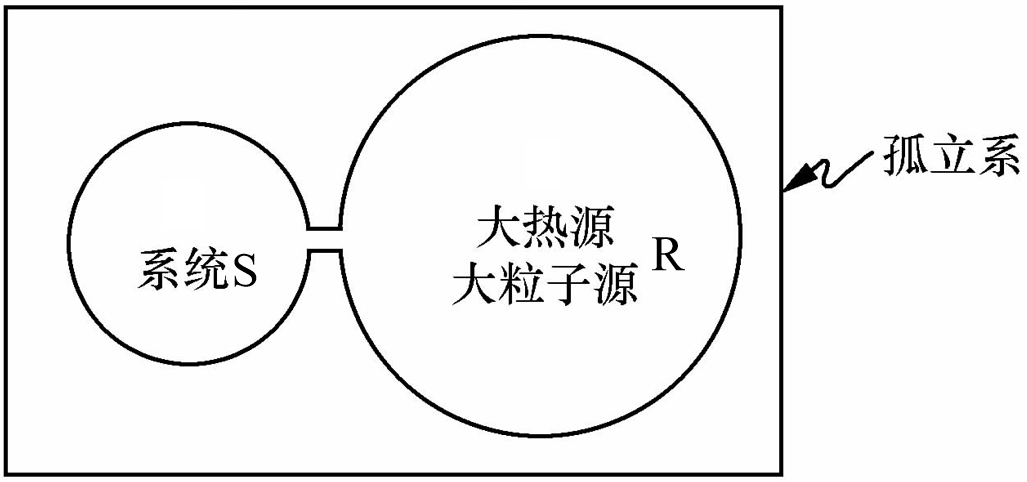
\includegraphics[scale=0.2]{gce.png}
	\caption{系统$S$和源$R$组成一个复合的孤立系。}
\end{figure}

假设系统与源之间的相互作用很弱,可以略去,则孤立系的能量和粒子数为
\begin{align}
E=E_s+E_r=const.\notag\\
N=N_s+N_r=const.
\end{align}
与正则系综相似,系统处于能量为$E_s$,粒子数为$N_s$状态的概率为
\begin{equation}\label{rs1}
\rho_s=\frac{W_r(N-N_s,E-E_s)}{W}
\end{equation}
同理,将$\ln W_r(N-N_s,E-E_s)$整体视作$\ln W_r(x,y)$在$x=N,y=E$处展开并忽略二次以上的小量,得到
\begin{align}
\ln W_r(N-N_s,E-E_s)&=\ln W_r(N,E)-N_s\biggl(\frac{\partial\ln W_r}{\partial N_r}\biggr)-E_s\bigg(\frac{\partial\ln W_r}{\partial E_r}\bigg)\notag\\
&=\ln W_r(N,E)-\alpha N_s-\beta E_s
\end{align}
将上式代入式\ref{rs1},合并与$N_s$和$E_s$无关的因子可得
\begin{equation}
\rho_s=\frac{1}{\Xi}e^{-\alpha N_s-\beta E_s}
\end{equation}
$\Xi$称为系统的巨配分函数,其值由概率的归一化条件确定(将求和时系统粒子数上限延拓至无穷大,以后用符号$N$表示$N_s$)
\begin{equation}
\Xi=\sum_{N=0}^{\infty}\sum_{s}e^{-\alpha N-\beta E_s}
\end{equation}
同理我们也可以改成对能级求和。设粒子数为$N$时,系统处于第$\ell$个能级的概率为(设简并度为$g_{\ell}$)
\begin{equation}
\rho_s=\frac{g_{\ell}}{\Xi}e^{-\alpha N-\beta E_{\ell}}
\end{equation}
巨配分函数为
\begin{equation}
\Xi=\sum_{N=0}^{\infty}\sum_{\ell}g_{\ell}e^{-\alpha N-\beta E_{\ell}}
\end{equation}
能级准连续时上式变为
\begin{equation}
\Xi=\sum_{N=0}^{\infty}\frac{e^{-\alpha N}}{h^{3N}N!}\int e^{-\beta E(\pmb{p},\pmb{q})}\dif\Omega
\end{equation}
\section{热力学量及其涨落}
巨正则系综中热力学量$\mathcal{O}$的统计平均值为
\begin{equation}
\aver{\mathcal{O}}=\frac{1}{\Xi}\sum_{N=0}^{\infty}\sum_{s}\mathcal{O}(N,E_s)e^{-\alpha N-\beta E_s}=\frac{1}{\Xi}\sum_{N=0}^{\infty}\sum_{\ell}\mathcal{O}(N,E_{\ell})g_{\ell}e^{-\alpha N-\beta E_{\ell}}
\end{equation}
能级准连续时上式变为
\begin{equation}
\aver{\mathcal{O}}=\frac{1}{\Xi}\sum_{N=0}^{\infty}\frac{e^{-\alpha N}}{h^{3N}N!}\int\mathcal{O}(\pmb{p},\pmb{q})e^{-\beta E(\pmb{p},\pmb{q})}\dif\Omega
\end{equation}
系统的平均能量为
\begin{equation}
\aver{E}=\frac{1}{\Xi}\sum_{N=0}^{\infty}\sum_{s}E_se^{-\alpha N-\beta E_s}=-\frac{\partial}{\partial\beta}\ln\Xi
\end{equation}
平均粒子数为
\begin{equation}\label{lizishu}
\aver{N}=\frac{1}{\Xi}\sum_{N=0}^{\infty}\sum_{s}Ne^{-\alpha N-\beta E_s}=-\frac{\partial}{\partial\alpha}\ln\Xi
\end{equation}
广义力为
\begin{equation}
\aver{Y_i}=\frac{1}{\Xi}\sum_{N=0}^{\infty}\sum_{s}\frac{\partial E_s}{\partial y_i}e^{-\alpha N-\beta E_s}=-\frac{1}{\beta}\frac{\partial\ln\Xi}{\partial y_i}
\end{equation}
因此压强为
\begin{equation}
p=\frac{1}{\beta}\frac{\partial\ln\Xi}{\partial V}
\end{equation}
用与正则系综中类似的方法可以得到熵为
\begin{equation}
S=\kb\biggl(\ln\Xi-\beta\frac{\partial\ln\Xi}{\partial\beta}-\alpha\frac{\partial\ln\Xi}{\partial\alpha}\biggr)=\kb(\ln\Xi+\beta\aver{E}+\alpha\aver{N})
\end{equation}
现在计算粒子数涨落
\begin{equation}
\aver{N^2}=\frac{1}{\Xi}\sum_{N=0}^{\infty}\sum_sN^2e^{-\alpha N-\beta E_s}=\frac{1}{\Xi}\frac{\partial^2\Xi}{\partial\alpha^2}=\biggl(\frac{\partial\ln\Xi}{\partial\alpha}\biggr)^2+\frac{\partial^2\ln\Xi}{\partial\alpha^2}
\end{equation}
上式第一项即为$\aver{N}^2$,所以粒子数涨落为
\begin{equation}
\sigma_N=\aver{N^2}-\aver{N}^2=\frac{\partial^2\ln\Xi}{\partial\alpha^2}=-\biggl(\frac{\partial\aver{N}}{\partial\alpha}\biggr)_{T,V}
\end{equation}
粒子数的相对涨落为
\begin{equation}
\frac{\sigma_N}{\aver{N}^2}=\frac{\partial}{\partial\alpha}\frac{1}{\aver{N}}
\end{equation}
与正则系综的情况类似,我们可以得到
\begin{equation}
\biggl(\frac{\partial\aver{E}}{\partial\beta}\biggr)_{\alpha,V}=-\aver{E^2}+\aver{E}^2=-\sigma_E
\end{equation}
能量的相对涨落为
\begin{equation}
\frac{\sigma_E}{\aver{E}^2}=\frac{\partial}{\partial\beta}\frac{1}{\aver{E}}
\end{equation}
将上述结果运用到单原子理想气体中,其巨配分函数为
\begin{align}\label{Xi}
\Xi&=\sum_{N=0}^{\infty}\frac{e^{-\alpha N}}{h^{3N}N!}\int\exp\biggl(-\beta \sum_{i=1}^{3N}\frac{p_i^2}{2m}\biggr)\dif\Omega\notag\\
&=\sum_{N=0}^{\infty}\frac{V^Ne^{-\alpha N}}{h^{3N}N!}\bigg(\frac{2\pi m}{\beta}\bigg)^{\frac{3N}{2}}\notag\\
&=\exp\biggl[\frac{V}{e^{\alpha}}\biggl(\frac{2\pi m}{\beta h^2}\biggr)^{3/2}\biggr]
\end{align}
由此可得单原子理想气体的平均粒子数、平均能量和压强分别为
\begin{align}\label{hehe}
\aver{N}&=-\frac{\partial}{\partial\alpha}\ln\Xi=\ln\Xi=\frac{V}{e^{\alpha}}\biggl(\frac{2\pi m}{\beta h^2}\biggr)^{3/2}\notag\\
\aver{E}&=-\frac{\partial}{\partial\beta}\ln\Xi=\frac32\aver{N}\kb T\notag\\
p&=\frac{1}{\beta}\frac{\partial\ln\Xi}{\partial V}=\frac{1}{\beta}\frac{\ln\Xi}{V}=\frac{\aver{N}}{V}\kb T
\end{align}
以及
\begin{align}
S&=\kb(\ln\Xi+\beta\aver{E}+\alpha\aver{N})\notag\\
&=\aver{N}\kb\alpha+\frac52\aver{N}\kb\notag\\
&=\aver{N}\kb\ln\biggl[\frac{V}{\aver{N}}\biggl(\frac{2\pi m}{\beta h^2}\biggr)^{3/2}\biggr]+\frac52\aver{N}\kb
\end{align}
这些都是我们熟知的结果。粒子数和能量的相对涨落为
\begin{equation}
\frac{\sigma_N}{\aver{N}^2}=\frac{\sigma_E}{\aver{E}^2}=\frac{1}{\aver{N}}
\end{equation}
因此对于实际系统来说其粒子数和能量的相对涨落都可忽略不计。
\section{F-D,B-E与M-B分布}
微观粒子可根据其自旋属性的不同分为费米子和玻色子,它们有着很不相同的统计性质。本节将导出这两种体系的粒子数按能量分布的规律,即费米-狄拉克分布和玻色-爱因斯坦分布,并讨论它们退化为玻尔兹曼分布的条件。假设系统的单粒子能级为$\varepsilon_i(i=0,1,2\cdots)$,简并度为$w_i$,占据单粒子能级$\varepsilon_i$的粒子数为$n_i$。各能级的粒子占据数构成一个序列,给出粒子按能级的分布,记为$\{n_i\}$。当系统处于粒子数为$N$,能级$E_{\ell}$上时,有如下关系(此处已假设粒子间不存在相互作用或者相互作用很弱可以略去,也就是说,本节的推导以及后面导出的F-D,B-E与M-B分布都只适用于这种由近独立子系组成的系统)
\begin{align}\label{sm}
N&=\sum_{i}n_i\notag\\
E_{\ell}&=\sum_{i}n_i\varepsilon_i
\end{align}
系统处于能级$E_{\ell}$上时的微观状态数$g_{\ell}$应为各单粒子能级上的微观状态数$k_i$的乘积,即
\begin{equation}
g_{\ell}=\prod_{i}k_i
\end{equation}
则系统处于能级$E_{\ell}$上的概率为
\begin{equation}
\rho_{\ell}=\frac{1}{\Xi}g_{\ell}e^{-\alpha N-\beta E_{\ell}}=\frac{1}{\Xi}\prod_{i}k_ie^{-\sum_{i}(\alpha+\beta\varepsilon_i)n_i}=\frac{1}{\Xi}\prod_{i}k_ie^{-(\alpha+\beta\varepsilon_i)n_i}
\end{equation}
巨配分函数为
\begin{align}
\Xi&=\sum_{N=0}^{\infty}\sum_{\ell}g_{\ell}e^{-\alpha N-\beta E_{\ell}}\notag\\
&=\sum_{N=0}^{\infty}\sum_{\ell}\prod_{i}k_ie^{-(\alpha+\beta\varepsilon_i)n_i}
\end{align}
上式求和$\sum_{\ell}$表示在给定粒子数$N$时,在满足式\ref{sm}的条件下,对所有的能级$E_{\ell}$求和。在巨正则系综中,由于系统的粒子数$N$可取从0到$\infty$的任何整数,所以对粒子数$N$和能级$E_{\ell}$求和时,各种分布$\{n_i\}$都能出现,因此,它等同于对所有可能的分布$\{n_i\}$的无约束求和,即(由于是对所有可能的分布$\{n_i\}$的无约束求和,所以求和与连乘可以互换)
\begin{equation}
\Xi=\sum_{\{n_i\}}\prod_{i}k_ie^{-(\alpha+\beta\varepsilon_i)n_i}=\prod_{i}\sum_{\{n_i\}}k_ie^{-(\alpha+\beta\varepsilon_i)n_i}=\prod_{i}\Xi_i
\end{equation}
其中
\begin{equation}\label{Xii}
\Xi_i=\sum_{\{n_i\}}k_ie^{-(\alpha+\beta\varepsilon_i)n_i}
\end{equation}
在各单粒子能级上的平均粒子数$\aver{n_i}$可以按求均值的公式求得
\begin{align}
\aver{n_i}&=\frac{1}{\Xi}\sum_{N=0}^{\infty}\sum_{\ell}n_ig_{\ell}e^{-\alpha N-\beta E_{\ell}}\notag\\
&=\frac{1}{\Xi}\sum_{\{n_i\}}n_i\biggl[\prod_{m}k_me^{-(\alpha+\beta\varepsilon_m)n_m}\biggr]
\end{align}
将上式方括号中$m=i$那一项记为$f_i$,剩下与$i$无关的内容记为$\phi$,则上式变为
\begin{align}
\aver{n_i}&=\frac{1}{\Xi}\phi\sum_{\{n_i\}}n_if_i\notag\\
&=\frac{1}{\Xi}\biggl[\prod_{m\neq i}k_me^{-(\alpha+\beta\varepsilon_m)n_m}\biggr]\biggl[\sum_{\{n_i\}}n_ik_ie^{-(\alpha+\beta\varepsilon_i)n_i}\biggr]\notag\\
&=\frac{1}{\Xi_i}\sum_{\{n_i\}}n_ik_ie^{-(\alpha+\beta\varepsilon_i)n_i}\notag\\
&=-\frac{\partial\ln\Xi_i}{\partial\alpha}
\end{align}
对于不同的粒子系统,$n_i$可能取的值不同,$k_i$也不同,因此必须考虑到不同粒子系统的不同统计方法。下面就费米、玻色和玻尔兹曼三种不同的统计系统导出其平均粒子数$\aver{n_i}$。
\\
\\
\leftline{\heiti 费米系统}
费米子受泡利不相容原理的约束,每个单粒子态最多可容纳一个粒子,对这类体系,单粒子能级
$\varepsilon_i$上分布的粒子数$n_i$必然少于能级的简并度$w_i$,即$n_i\leq w_i$,因此该单粒子能级的微观状态数应为在$w_i$个单粒子态中挑选$n_i$个放上粒子的组合数,即
\begin{equation}
k_i=C_{w_i}^{n_i}=\frac{w_i!}{n_i!(w_i-n_i)!}
\end{equation}
根据式\ref{Xii}其$\Xi_i$为
\begin{equation}
\Xi_i=\sum_{n_i=0}^{w_i}\frac{w_i!}{n_i!(w_i-n_i)!}e^{-(\alpha+\beta\varepsilon_i)n_i}=(1+e^{-(\alpha+\beta\varepsilon_i)})^{w_i}
\end{equation}
上式的推导用到了二项式定理\footnote{$(1+x)^m=\sum_{n=0}^{m}\frac{m!}{n!(m-n)!}x^n$}。则平均粒子数为
\begin{equation}
\aver{n_i}=-\frac{\partial\ln\Xi_i}{\partial\alpha}=\frac{w_i}{e^{\alpha+\beta\varepsilon_i}+1}
\end{equation}
\leftline{\heiti 玻色系统}
玻色子不受泡利不相容原理的约束,允许任意多个粒子占据一个单粒子态。为便于分析,如下图所示,我们用$w_i$个盒子$\square$代表单粒子态,用$n_i$个圆圈$\bigcirc$表示粒子,将单粒子态和粒子混排成一个序列,并要求最左边的一个是盒子。不同的排列给出不同的序列,每一序列可代表粒子填充单粒子态的一种方式,具体理解是:两盒子之间的粒子填入其左边最近邻的盒子(单粒子态),单粒子态按盒子在序列中的位置编号。
\begin{figure}[ht]
	\centering
	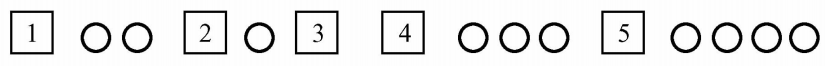
\includegraphics[scale=0.3]{boson.png}
	\caption{玻色子状态和粒子序列。}
\end{figure}

因为盒子和圆圈的放置是任意的,因此该单粒子能级的微观状态数应为在剩下的$w_i+n_i-1$个位置上选$n_i$个放上粒子的组合数,即
\begin{equation}
k_i=C_{w_i+n_i-1}^{n_i}=\frac{(w_i+n_i-1)!}{n_i!(w_i-1)!}
\end{equation}
根据式\ref{Xii}其$\Xi_i$为
\begin{equation}
\Xi_i=\sum_{n_i=0}^{\infty}\frac{(w_i+n_i-1)!}{n_i!(w_i-1)!}e^{-(\alpha+\beta\varepsilon_i)n_i}=(1-e^{-(\alpha+\beta\varepsilon_i)})^{-w_i}
\end{equation}
上式的推导用到了$(1-x)^{-m}$的泰勒展开\footnote{$(1-x)^{-m}=\sum_{n=0}^{\infty}\frac{(m+n-1)!}{n!(m-1)!}x^n$}。则平均粒子数为
\begin{equation}\label{bs}
\aver{n_i}=-\frac{\partial\ln\Xi_i}{\partial\alpha}=\frac{w_i}{e^{\alpha+\beta\varepsilon_i}-1}
\end{equation}
\leftline{\heiti 退化条件}
我们惊讶地发现,上面两种系统的单粒子能级平均粒子数差异只在分母的$\pm1$,即
\begin{equation}
\aver{n_i}=\frac{w_i}{e^{\alpha+\beta\varepsilon_i}\pm1}
\end{equation}
当$e^{\alpha+\beta\varepsilon_i}\gg1$时,这个$\pm1$的差异不再显著,上述分布退化为
\begin{equation}
\aver{n_i}=w_ie^{-(\alpha+\beta\varepsilon_i)}
\end{equation}
这样的分布称之为麦克斯韦-玻尔兹曼分布。这一退化条件对所有能级都成立,特别是对最低能级$\varepsilon_0$也成立,不失一般性,可选取$\varepsilon_0=0$,则$e^{\alpha+\beta\varepsilon_i}\gg1$的充分条件是
\begin{equation}
e^{\alpha}\gg1
\end{equation}
上式称为非简并条件,它的等效形式是
\begin{equation}
\frac{\aver{n_i}}{w_i}\ll1
\end{equation}
上式表示在每个单粒子态上的平均粒子数远小于1,这就是说,绝大多数的量子态都是空的,有两个及以上的粒子处在同一单粒子态的概率极小,泡利不相容原理无需考虑。以单原子理想气体为例,由\ref{hehe}第一式可得
\begin{equation}
e^{\alpha}=\frac{V}{N}\biggl(\frac{2\pi m}{\beta h^2}\biggr)^{3/2}=\frac1n\biggl(\frac{2\pi m\kb T}{h^2}\biggr)^{3/2}
\end{equation}
也就是说,$e^{\alpha}\gg1$实际上是高温和低密度极限,在这种极限下费米-狄拉克分布和玻色-爱因斯坦分布都退化到麦克斯韦-玻尔兹曼分布。非简并条件还可以用另一种形式来表述
\begin{equation}
\aver{d}=\biggl(\frac{V}{N}\biggr)^{1/3}\gg\lambda_T\equiv\frac{h}{\sqrt{2\pi m\kb T}}
\end{equation}
$\aver{d}$表示两粒子平均间距,$\lambda_T$定义为粒子热运动的德布罗意波长,则上式表明粒子间距远大于粒子热运动的德布罗意波长,此时粒子作为波包而言彼此之间的重叠完全可以忽略,粒子波动性可以不予考虑,全同性也不再重要。
\chapter{一些实际应用}
\section{声子气}
本节用玻色统计理论处理固体热容问题。固体中相邻原子间距很小,原子间相互作用很强,每个原子只能在其平衡位置附近做微振动。设一固体由$N$个原子组成,其运动自由度则为$3N$。在研究晶格的小振动时,可利用简正变换,用$3N$个简正坐标来描述其振动,称为简正振动。按照量子理论,这$3N$个振动频率为$w_i(i=1,2,\cdots,3N)$的简正振动的能量是量子化的,即
\begin{equation}
E=\sum_{i=1}^{3N}\hbar w_i(n_i+\frac12)
\end{equation}
其中,$n_i$是描述第$i$个简正振动的量子数。这$3N$个简正振动模式中每一个都对应着晶格点阵中传播的一种振动波,因此可以用波矢$\pmb{k}_i$和偏振方向来区分它们。可以把简正振动的能量量子看成一种准粒子,称为声子,因此这样的系统也被称为声子气。第$i$个简正振动对应的声子的准动量$\pmb{p}_i$和能量分别为
\begin{equation}
\pmb{p}_i=\hbar\pmb{k}_i\qquad \varepsilon_i=\hbar w_i
\end{equation}
对于第$i$个简正振动,其能量为$\hbar w_i(n_i+\frac12)$,相当于产生了$n_i$个能量为$\hbar w_i$,准动量为$\hbar\pmb{k}_i$的声子。由于$n_i$可取任意非负整数,即处于该状态的声子数是任意的,因此声子遵循玻色分布。从微观上看,在平衡态下各简正振动的能量不断变化,相当于各种状态的声子不断被产生和湮灭,声子数并不恒定,因此声子的化学势$\mu=0$。由式\ref{bs}得温度为$T$时能量为$\hbar w$的平均声子数为
\begin{equation}
\aver{n}=\frac{1}{e^{\beta\hbar w}-1}
\end{equation}
因此
\begin{equation}\label{energy}
E=\sum_{i=1}^{3N}\hbar w_i(\aver{n_i}+\frac12)=E_0+\sum_{i=1}^{3N}\frac{\hbar w_i}{e^{\beta\hbar w_i}-1}
\end{equation}
其中,$E_0=\sum_{i=1}^{3N}\frac12\hbar w_i$是简正振子零点能之和,对热容无贡献可略去。若要求出固体热运动的能量,需要知道这$3N$个简正振动的频率。我们先看看固体热容的经典处理方法,然后介绍两种频谱模型——爱因斯坦模型和德拜模型。
\\
\\
\leftline{\heiti 经典方法}
用经典力学描述每一个简正振子,其能量为
\begin{equation}
\varepsilon=\frac{p^2}{2m}+\frac12mw^2q^2
\end{equation}
上式包含两个平方项,根据能均分定理知其平均能量为$\kb T$,则系统的总能量为$3N\kb T$,于是热容为
\begin{equation}
C_V=3N\kb
\end{equation}
上式即为杜隆-珀蒂定律。这个结果在高温情况下与实验结果符合得很好,但在低温情形与实验结果严重偏离。固体热容在低温下的实验结果为:对于金属固体,$C_V\propto T$;对于非金属固体,$C_V\propto T^3$。
\\
\\
\leftline{\heiti 爱因斯坦模型}
爱因斯坦假设这$3N$个简正振动的频率都相同,记为$w_e$,称为爱因斯坦特征频率。因此
\begin{equation}
E=3N\frac{\hbar w_e}{e^{\beta\hbar w_e}-1}
\end{equation}
故有
\begin{equation}
C_V=\frac{\partial E}{\partial T}=3N\kb\biggl(\frac{\hbar w_e}{\kb T}\biggr)^2\frac{e^{\hbar w_e/\kb T}}{(e^{\hbar w_e/\kb T}-1)^2}
\end{equation}
记$\hbar w_e=\kb\theta_e$,其中$\theta_e$称为爱因斯坦特征温度\footnote{爱因斯坦特征频率$w_e$可由固体的弹性常数、杨氏模量、原子质量和晶格常数定出,从而确定爱因斯坦特征温度$\theta_e$}。上式可改写为
\begin{equation}
C_V=3N\kb\biggl(\frac{\theta_e}{T}\biggr)^2\frac{e^{\theta_e/T}}{(e^{\theta_e/T}-1)^2}
\end{equation}
现在考查上式的极限情形。对于高温极限,即$T\gg\theta_e$,我们有$e^{\theta_e/T}-1\approx\theta_e/T$,则上式化为
\begin{equation}
C_V=3N\kb
\end{equation}
此式与杜隆-珀蒂定律一致。现在来看低温极限,即$T\ll\theta_e$,我们有$e^{\theta_e/T}-1\approx e^{\theta_e/T}$,此时热容为
\begin{equation}
C_V=3N\kb\biggl(\frac{\theta_e}{T}\biggr)^2e^{-\theta_e/T}
\end{equation}
不难看出,当$T\rightarrow0$时,$C_V$随温度以指数趋于零,与实验结果不符,原因是其频谱模型过于简单,关于所有振子以相同频率振动的假设与实际情况偏差较大。
\\
\\
\leftline{\heiti 德拜模型}
德拜提出假设:联系晶格振动的$3N$个简正模式为一系列低频振动,其在固体中传播的波长远大于晶格常数,可以将固体视为连续介质,$3N$个简正振动即可看作弹性波。弹性波分为纵波和横波,纵波有一个振动方向,横波有两个独立的偏振方向。给定偏振方向的一种弹性波的波矢在$k\sim k+\dif k$范围内的振动模式数为\footnote{一个自由粒子在体积元$\dif p_x\dif p_y\dif p_z\dif x\dif y\dif z$中可能的微观状态数应为
\[\frac{1}{h^3}\dif p_x\dif p_y\dif p_z\dif x\dif y\dif z\]
将体积积分,得到在体积$V$内,动量在$\pmb{p}\sim\pmb{p}+\dif\pmb{p}$范围内的微观状态数为
\[\frac{V}{h^3}\dif p_x\dif p_y\dif p_z\]
因此动量的绝对值在$p\sim p+\dif p$范围内的微观状态数为
\[\frac{4\pi V}{h^3}p^2\dif p\]
将$p=\hbar k$代入上式得到波矢在$k\sim k+\dif k$范围内的微观状态数为
\[\frac{Vk^2}{2\pi^2}\dif k\]
}
\begin{equation}\label{weiqu}
\frac{Vk^2}{2\pi^2}\dif k
\end{equation}
由弹性波理论可知纵波与横波分别满足以下关系
\begin{equation}
w_l=c_lk\qquad w_t=c_tk
\end{equation}
其中$c_l$和$c_t$分别为纵波和横波的波速。将上式代入式\ref{weiqu},并计入横波的两个独立的偏振方向,便得到频率在$w\sim w+\dif w$范围内的振动模式数为
\begin{equation}
D(w)\dif w=\frac{V}{2\pi^2}\biggl(\frac{1}{c_l^3}+\frac{2}{c_t^3}\biggr)w^2\dif w=Bw^2\dif w
\end{equation}
由于振动模式总数为$3N$,故而$w$应有一上限,记为$w_d$,称为德拜频率,由上式得
\begin{equation}
\int_{0}^{w_d}Bw^2\dif w=3N
\end{equation}
所以
\begin{equation}
w_d=\biggl(\frac{9N}{B}\biggr)^{1/3}
\end{equation}
因此式\ref{energy}可由求和变为积分
\begin{equation}
E=\int_{0}^{w_d}\frac{\hbar w}{e^{\beta\hbar w}-1}D(w)\dif w=\frac{9N}{w_d^3}\int_{0}^{w_d}\frac{\hbar w^3}{e^{\beta\hbar w}-1}\dif w
\end{equation}
令$y=\hbar w/\kb T$和$x=\hbar w_d/\kb T=\theta_d/T$,其中$\theta_d$称为德拜特征温度,则上式变为
\begin{equation}
E=3N\kb T\frac{3}{x^3}\int_{0}^{x}\frac{y^3}{e^y-1}\dif y=3N\kb T\mathcal{D}(x)
\end{equation}
其中
\begin{equation}
\mathcal{D}(x)=\frac{3}{x^3}\int_{0}^{x}\frac{y^3}{e^y-1}\dif y
\end{equation}
下面讨论两种极限情形,对于高温极限,即$T\gg\theta_d$,有$e^y-1\approx y$,则$\mathcal{D}(x)\approx1$,于是$C_V=3N\kb$,与杜隆-珀蒂定律一致。对于低温极限,即$T\ll\theta_d$,此时$x\gg1$,可将上式的积分上限取为无穷大,即
\begin{equation}
\mathcal{D}(x)\approx\frac{3}{x^3}\int_{0}^{\infty}\frac{y^3}{e^y-1}\dif y=\frac{\pi^4}{5}\biggl(\frac{T}{\theta_d}\biggr)^3
\end{equation}
上式中的定积分结果为$\pi^4/15$,可由积分表查到。于是得
\begin{equation}
C_V=3N\kb\frac{4\pi^4}{5}\biggl(\frac{T}{\theta_d}\biggr)^3\propto T^3
\end{equation}
上式与非金属固体的热容实验结果吻合,但与金属固体的实验结果有较大偏差。为了获得与实验完全相符的理论结果,还应考虑金属中电子的热容,具体计算见\ref{jinshu}节。
\section{光子气}
只吸收电磁波而不向外界辐射的物体称为黑体。空腔为典型的黑体,当腔内辐射与吸收达到平衡时,空腔的器壁不断发射和吸收光子,光子数是不守恒的,因此光子气的化学势$\mu=0$。光子自旋为1,是玻色子,服从玻色分布,因此
\begin{align}\label{kaiwanxiao}
\aver{n_i}&=\frac{w_i}{e^{\beta\varepsilon_i}-1}\notag\\
\ln\Xi&=-\sum_iw_i\ln(1-e^{-\beta\varepsilon_i})
\end{align}
考虑到光子的两个独立的偏振方向,则光子气体的动量在$p\sim p+\dif p$范围内的微观状态数为
\begin{equation}
g(p)\dif p=2\frac{4\pi V}{h^3}p^2\dif p
\end{equation}
光子能量为$\varepsilon=h\nu$,则$p=\varepsilon/c=h\nu/c$,代入上式得频率在$\nu\sim\nu+\dif\nu$范围内的微观状态数为
\begin{equation}
g(\nu)\dif\nu=\frac{8\pi V}{c^3}\nu^2\dif\nu
\end{equation}
于是\ref{kaiwanxiao}第二式可由求和变为积分,即
\begin{equation}\label{aye}
\ln\Xi=-\int_{0}^{\infty}\ln(1-e^{-\beta h\nu})g(\nu)\dif\nu=-\frac{8\pi V}{c^3}\int_{0}^{\infty}\ln(1-e^{-\beta h\nu})\nu^2\dif\nu
\end{equation}
于是光子气体的总能量为
\begin{equation}
\aver{E}=-\frac{\partial\ln\Xi}{\partial\beta}=\frac{8\pi V}{c^3}\int_{0}^{\infty}\frac{h\nu^3}{e^{\beta h\nu}-1}\dif\nu
\end{equation}
总能量可以表示为能量谱密度的积分,$E=\int_{0}^{\infty}E_{\nu}\dif\nu$,与上式比较得到能量谱密度为
\begin{equation}
E_{\nu}\dif\nu=\frac{8\pi V}{c^3}\frac{h\nu^3}{e^{\beta h\nu}-1}\dif\nu
\end{equation}
上式即为黑体辐射的普朗克公式。下面对普朗克公式做一些讨论,首先看看极限情况,低频时$e^{\beta h\nu}-1\approx\beta h\nu$,普朗克公式退化为瑞利-金斯公式
\begin{equation}
E_{\nu}\dif\nu=\frac{8\pi V}{c^3}\nu^2\kb T\dif\nu
\end{equation}
高频时,$e^{\beta h\nu}\gg1$,可忽略普朗克公式分母中的$-1$,此时退化为维恩公式
\begin{equation}
E_{\nu}\dif\nu=\frac{8\pi V}{c^3}h\nu^3e^{-h\nu/\kb T}\dif\nu
\end{equation}
将$\nu=c/\lambda$代入普朗克公式可求得能量按波长的分布
\begin{equation}
E_{\lambda}\dif\lambda=\frac{8\pi Vhc}{\lambda^5}\frac{1}{e^{hc/\lambda\kb T}-1}\dif\lambda
\end{equation}
能量按波长分布有一峰值,此时的波长$\lambda_m$满足条件$(\frac{\dif E_{\lambda}}{\dif\lambda})|_{\lambda=\lambda_m}=0$,得
\begin{equation}
1-\frac{x_m}{5}-e^{-x_m}=0
\end{equation}
其中$x_m=\frac{hc}{\kb T\lambda_m}$,数值解得$x_m\approx4.965114$,故得
\begin{equation}
\lambda_mT=0.28978\ \text{cm}\cdot\text{K}
\end{equation}
此即维恩位移定律。它告诉我们,当辐射场的温度升高时,$\lambda_m$向短波移动。这一定律可以用来测温,由实验观测数据得到$\lambda_m$后即可估算温度。事实上式\ref{aye}可以精确计算,即
\begin{align}
\ln\Xi&=-\frac{8\pi V}{c^3}\int_{0}^{\infty}\ln(1-e^{-\beta h\nu})\nu^2\dif\nu\notag\\
\stackrel{\text{令$x=\beta h\nu$}}{=}&-\frac{8\pi V}{h^3c^3\beta^3}\int_{0}^{\infty}\ln(1-e^{-x})x^2\dif x\notag\\
&=-\frac{8\pi V}{h^3c^3\beta^3}\biggl[\frac{x^3}{3}\ln(1-e^{-x})\bigg|_0^{\infty}-\frac13\int_{0}^{\infty}\frac{x^3}{e^{x}-1}\dif x\biggr]\notag\\
&=\frac{1}{45}\frac{\pi^2 V}{\hbar^3c^3\beta^3}
\end{align}
上式第三行方括号中第一项为零。则辐射场的总能量为
\begin{equation}
\aver{E}=-\frac{\partial\ln\Xi}{\partial\beta}=\frac{\pi^2\kb^4}{15\hbar^3c^3}VT^4
\end{equation}
由此可见,辐射场的总能量与绝对温度的四次方成正比。由此还可导出斯特藩-玻尔兹曼定律、光压表达式、光子气的熵和热容等,此处不再赘述。下面来计算平均光子数$\aver{N}$,由于化学势$\mu=0$,不能直接用式\ref{lizishu},但可以从式\ref{sm}出发来求,即
\begin{align}
\aver{N}&=\int_{0}^{\infty}\frac{1}{e^{\beta h\nu}-1}g(\nu)\dif\nu\notag\\
&=\frac{8\pi V}{c^3}\int_{0}^{\infty}\frac{\nu^2}{e^{\beta h\nu}-1}\dif\nu\notag\\
\stackrel{\text{令$x=\beta h\nu$}}{=}&\frac{8\pi V}{\beta^3h^3c^3}\int_{0}^{\infty}\frac{x^2}{e^{x}-1}\dif x\notag\\
&=16\pi V\zeta(3)\biggl(\frac{\kb T}{hc}\biggr)^3
\end{align}
上式第三行的定积分结果为$2\zeta(3)$,可由积分表查到,其中$\zeta(\nu)$为黎曼$\zeta$函数,且$\zeta(3)\approx1.202$。则辐射场中单光子的平均能量为
\begin{equation}
\aver{\varepsilon}=\frac{\aver{E}}{\aver{N}}=\frac{\pi^4}{30\zeta(3)}\kb T\approx2.7\kb T
\end{equation}
\section{BEC}
本节讨论玻色-爱因斯坦凝聚问题。根据式\ref{bs}知道玻色气体原子按能级的分布为
\begin{equation}
\aver{n_i}=\frac{w_i}{e^{\beta(\varepsilon_i-\mu)}-1}
\end{equation}
因为$\aver{n_i}\ge0$,所以$\varepsilon_i\ge\mu$。不失一般性,可选取基态为能量零点,即$\varepsilon_0=0$,因此$\mu\le0$。由$\varepsilon=p^2/2m$可得能量在$\varepsilon\sim\varepsilon+\dif\varepsilon$范围内的粒子数为(忽略自旋带来的简并度)
\begin{equation}
\frac{4\pi V}{h^3}p^2\dif p=\frac{2\pi V}{h^3}(2m)^{3/2}\sqrt{\varepsilon}\dif\varepsilon
\end{equation}
因此总粒子数为
\begin{equation}
N=\sum_{i}\frac{w_i}{e^{\beta(\varepsilon_i-\mu)}-1}=\frac{2\pi V}{h^3}(2m)^{3/2}\int_{0}^{\infty}\frac{\sqrt{\varepsilon}\dif\varepsilon}{e^{\beta(\varepsilon-\mu)}-1}
\end{equation}
必须指出的是,上面将求和变为积分时,由于因子$\sqrt{\varepsilon}$使得基态($\varepsilon=0$)被忽略。当温度不很低的时候,基态上的粒子很少,这样的计算是正确的。但当温度很低时,由于没有泡利不相容原理的限制,粒子向基态聚集,使得基态粒子数$N_0$对求和的贡献不可忽略,即
\begin{equation}\label{nanding}
N=N_0+\frac{2\pi V}{h^3}(2m)^{3/2}\int_{0}^{\infty}\frac{\sqrt{\varepsilon}\dif\varepsilon}{e^{\beta(\varepsilon-\mu)}-1}
\end{equation}
考虑将体系降温,化学势$\mu$必然增大,直至降到某一临界温度$T_c$时,化学势$\mu=0$(事实上是小于但非常接近于零),且当温度继续下降时化学势为零保持不变。这一临界温度可由下式确定
\begin{equation}
\frac{N}{V}=\frac{2\pi}{h^3}(2m)^{3/2}\int_{0}^{\infty}\frac{\sqrt{\varepsilon}\dif\varepsilon}{e^{\varepsilon/\kb T_c}-1}
\end{equation}
引入变量$x=\varepsilon/\kb T_c$,则上式变为
\begin{equation}
\frac{N}{V}=\biggl(\frac{2\pi m\kb T_c}{h^2}\biggr)^{3/2}\frac{2}{\sqrt{\pi}}\int_{0}^{\infty}\frac{\sqrt{x}\dif x}{e^x-1}
\end{equation}
上式中的定积分可由积分表查到,其结果为
\begin{equation}
\frac{2}{\sqrt{\pi}}\int_{0}^{\infty}\frac{\sqrt{x}\dif x}{e^x-1}\approx2.612
\end{equation}
因此
\begin{equation}\label{tc}
T_c=\frac{h^2}{2\pi m\kb}\biggl(\frac{N}{2.612V}\biggr)^{2/3}
\end{equation}
当$T<T_c$时,化学势$\mu=0$,此时式\ref{nanding}变为
\begin{equation}
N=N_0+2.612V\biggl(\frac{2\pi m\kb T}{h^2}\biggr)^{3/2}
\end{equation}
将式\ref{tc}代入上式可得
\begin{equation}
\frac{N_0}{N}=1-\biggl(\frac{T}{T_c}\biggr)^{3/2}
\end{equation}
上式表明,温度高于$T_c$时,基态粒子数$N_0$与粒子总数相比可忽略不计。当系统冷却至$T_c$时,其行为发生明显的转变:$N_0/N$急剧增大。这种转变是一种相变。在相变点$T_c$,系统由粒子弥散在各能级的状态转变为在最低能级(动量为零的态)聚集的状态。不过,这种凝聚是粒子在动量空间的凝聚,只能在不受泡利不相容原理限制的玻色气体中发生。

在临界温度附近,玻色气体的热力学函数表现出十分特别的性质,这些性质中最具代表意义的是热容的变化。下面我们简要讨论玻色气体的热容。对$T<T_c$情形,总能量为
\begin{align}
E&=\frac{2\pi V}{h^3}(2m)^{3/2}\int_{0}^{\infty}\frac{\varepsilon^{3/2}\dif\varepsilon}{e^{\beta\varepsilon}-1}\notag\\
&=\frac{2\pi V}{h^3}(2m)^{3/2}(\kb T)^{5/2}\int_{0}^{\infty}\frac{x^{3/2}\dif x}{e^{x}-1}\notag\\
&=0.77N\kb\frac{T^{5/2}}{T_c^{3/2}}
\end{align}
上式第二行的定积分可由积分表查到,其结果约为1.783。则热容为
\begin{equation}
C_V=1.925N\kb\biggl(\frac{T}{T_c}\biggr)^{3/2}
\end{equation}
临界温度时热容为$C_V=1.925N\kb$。随着温度的降低,热容以温度的3/2次方的规律下降,直至温度趋于绝对零度时趋于零。在高温情形,玻色气体趋于经典的理想气体,其热容可通过能均分定理得到
\begin{equation}
C_V=\frac32N\kb
\end{equation}
明显低于临界温度时的热容。根据以上分析,我们可以定性地画出理想玻色气体热容对温度变化的曲线,如图所示。理想玻色气体的热容在温度较高时遵从杜隆-珀蒂定律;随着温度降低而接近临界温度时,热容迅速增大,至$T=T_c$时取极大值;若温度继续降低,热容又以3/2次幂律下降。在临界点附近,热容对温度的依赖性质发生突变,表现出明显的相变特征。临界温度$T_c$将理想玻色气体分隔为两个不同的相。温度低于$T_c$的相为凝聚相。图中的热容曲线呈$\lambda$形,所以常将此类相变称为$\lambda$相变。
\begin{figure}[ht]
	\centering
	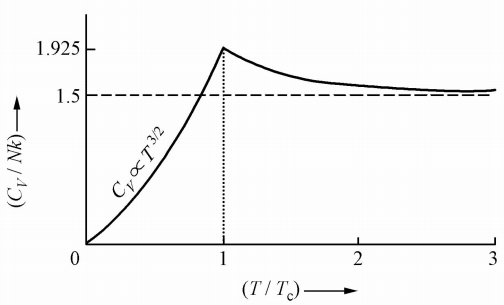
\includegraphics[scale=0.5]{cv.png}
	\caption{理想玻色气体热容随温度的变化。}
\end{figure}

需要特别指出的是,如前所述,玻色-爱因斯坦凝聚出现在化学势$\mu$由小于零而趋于零处,因此对于化学势$\mu$恒为零的玻色体系,例如光子气,玻色-爱因斯坦凝聚不存在。
\clearpage
\section{自由电子气}\label{jinshu}
金属中的电子是最典型的费米子。作为初级近似,可以略去电子之间的相互作用,将其视为理想费米气体。本节将用费米统计研究这种体系的热力学性质,并主要关注其热容。

考虑到电子的两个自旋取向,则能量处于$\varepsilon\sim\varepsilon+\dif\varepsilon$范围内的电子态的数目为
\begin{equation}
g(\varepsilon)\dif\varepsilon=\frac{4\pi V}{h^3}(2m)^{3/2}\sqrt{\varepsilon}\dif\varepsilon
\end{equation}
下面分零温与非零温两种情况讨论。
\\
\\
\leftline{\heiti 绝对零度时的电子气}
在$T=0$时,电子从最低能级$\varepsilon=0$开始按每能级两个逐级填充,直至全部填完,最高能级为$\mu_0$,再往上的能级全部空着。总电子数守恒的条件为
\begin{equation}
N=\int_{0}^{\mu_0}g(\varepsilon)\dif\varepsilon=\frac{4\pi V}{h^3}(2m)^{3/2}\int_{0}^{\mu_0}\sqrt{\varepsilon}\dif\varepsilon=\frac{8\pi V}{3h^3}(2m)^{3/2}\mu_0^{3/2}
\end{equation}
由此可解出$\mu_0$作为粒子数$N$的函数
\begin{equation}
\mu_0=\frac{h^2}{8m}\biggl(\frac{3N}{\pi V}\biggr)^{2/3}
\end{equation}
$\mu_0$又称为费米能级,记作$\varepsilon_f$。它所对应的动量记作$p_f$,称为费米动量。根据自由电子的能动量关系$\varepsilon=p^2/2m$我们知道,此时电子在动量空间所占据的区域是一个半径为费米动量的球,称为费米球或费米海,球的表面又称为费米面。费米动量为
\begin{equation}
p_f=\sqrt{2m\varepsilon_f}=h\biggl(\frac{3N}{8\pi V}\biggr)^{1/3}
\end{equation}
$T=0$时电子气的总能量为
\begin{equation}
E=\int_{0}^{\mu_0}\varepsilon g(\varepsilon)\dif\varepsilon=\frac35N\mu_0
\end{equation}
因此电子的平均能量为
\begin{equation}
\aver{\varepsilon}=\frac35\mu_0
\end{equation}
这就是说,费米气体的基态能量并不为零。这是由于泡利不相容原理带来了排斥作用,导致电子即使在绝对零度时仍在做激烈运动,容易估算出此时电子的平均速率约为$10^6\text{m/s}$。
\\
\\
\leftline{\heiti 非零温情况}
先计算巨配分函数的对数
\begin{equation}
\ln\Xi=\frac{4\pi V}{h^3}\biggl(\frac{2m}{\beta}\biggr)^{3/2}\int_{0}^{\infty}\ln(1+e^{-\alpha-x})\sqrt{x}\dif x
\end{equation}
这里已引入了变换$x=\beta\varepsilon$,通过一系列的近似可将上式求出,从而得到系统的热力学量,此处不再赘述。系统的粒子数和能量为
\begin{align}
N&=\frac{4\pi V}{h^3}(2m)^{3/2}\int_{0}^{\infty}\frac{\sqrt{\varepsilon}\dif\varepsilon}{e^{\beta(\varepsilon-\mu)}+1}\notag\\
E&=\frac{4\pi V}{h^3}(2m)^{3/2}\int_{0}^{\infty}\frac{\varepsilon^{3/2}\dif\varepsilon}{e^{\beta(\varepsilon-\mu)}+1}
\end{align}
为计算这两个式子,考虑如下形式的积分
\begin{equation}
I=\int_{0}^{\infty}\frac{\eta(\varepsilon)\dif\varepsilon}{e^{\beta(\varepsilon-\mu)}+1}
\end{equation}
索末菲证明,在低温下,上式可以展开为
\begin{equation}
I=\int_{0}^{\mu}\eta(\varepsilon)\dif\varepsilon+\frac{\pi^2}{6\beta^2}\eta'(\mu)+\cdots
\end{equation}
因此
\begin{align}
N&=\frac{8\pi V}{3h^3}(2m\mu)^{3/2}\biggl(1+\frac{\pi^2}{8\beta^2\mu^2}\biggr)\notag\\
E&=\frac{8\pi V}{5h^3}(2m\mu)^{3/2}\biggl(1+\frac{5\pi^2}{8\beta^2\mu^2}\biggr)
\end{align}
理论上可由上面的第一式求出化学势,但由于方程较复杂,只能近似求解。将该式化为
\begin{equation}
\mu=\mu_0\biggl(1+\frac{\pi^2}{8\beta^2\mu^2}\biggr)^{-2/3}
\end{equation}
因为$\mu\gg\kb T$,上式括号中的分数项可略去,由此得到化学势的一级近似$\mu=\mu_0$,再将一级近似代回上式右边并利用$(1+x)^{-a}\sim(1-ax)$可得
\begin{equation}
\mu=\mu_0\biggl(1-\frac{\pi^2}{12\beta\mu_0^2}\biggr)
\end{equation}
所以系统能量为
\begin{equation}
E=\frac35N\mu_0+\frac{\pi^4}{4}N\frac{\kb^2T^2}{\mu_0}
\end{equation}
电子热容为
\begin{equation}
C_V=\frac{\pi^2}{2}N\kb^2\frac{T}{\mu_0}\propto T
\end{equation}
所以在通常的温度下,电子气的热容很小,和声子气的热容相比可以忽略不计。然而,在很低的温度下,情况便不同了。在低温下,金属中晶格振动的热容随温度的三次方趋于零,而电子气的热容随温度的一次方趋于零,因此在极低的温度下,电子气对热容的贡献成为主要的了。
\appendix
\chapter{$3N$维单位球体积的计算}\label{vo}
为了计算$K$值,我们来计算以下积分(式中$E=\sum_{i=1}^{3N}\frac{p_i^2}{2m}$)
\[
I=\frac{1}{h^{3N}N!}\int e^{-\beta E}\dif\Omega
\]
法一:直接积分,即
\[
I=\frac{V^N}{h^{3N}N!}\prod_{i=1}^{3N}\int_{-\infty}^{+\infty}e^{-\beta\frac{p_i^2}{2m}}\dif p_i=\frac{V^N}{h^{3N}N!}\biggl(\frac{2\pi m}{\beta}\biggr)^{3N/2}
\]
上式运用了高斯积分公式$\int_{-\infty}^{+\infty}e^{-\alpha x^2}\dif x=\sqrt{\pi/\alpha}$

\leftline{法二:}
\begin{align}
I&=\int_{0}^{\infty}e^{-\beta E}\dif\Sigma\notag\\
&=\int_{0}^{\infty}e^{-\beta E}\frac{\partial\Sigma}{\partial E}\dif E\notag\\
&=K\frac{3N}{2}\frac{V^N}{h^{3N}N!}(2m)^{\frac{3N}{2}}\int_{0}^{\infty}e^{-\beta E}E^{\frac{3N}{2}-1}\dif E\notag\\
&=K\frac{V^N}{h^{3N}N!}\biggl(\frac{2m}{\beta}\biggr)^{\frac{3N}{2}}\Gamma(\frac{3N}{2}+1)\notag
\end{align}
上式运用了$\Gamma$函数的定义$\Gamma(\alpha)=\int_{0}^{\infty}x^{\alpha-1}e^{-x}\dif x$及其性质$\Gamma(\alpha+1)=\alpha\Gamma(\alpha)$。比较两种方法得到的积分值可得
\[
K=\frac{\pi^{\frac{3N}{2}}}{\Gamma(\frac{3N}{2}+1)}
\]


























































































































\begin{thebibliography}{99}
	
	\bibitem{T. D. Lee} 
	李政道,《统计力学》,上海科学技术出版社, 2006.
	
	\bibitem{kardar}
	Mehran Kardar, \emph{Statistical Physics of Particles}, Cambridge University Press, 2007.
	
	\bibitem{kardar}
	Walter Greiner \emph{et al.}, \emph{Thermodynamics and Statistical Mechanics}, Springer, 1995.
	
	\bibitem{liangxixia} 
	刘川,平衡态统计物理v2.33,课程讲义, 2014.
	
	\bibitem{liangxixia} 
	梁希侠,《统计热力学》(第三版),科学出版社, 2016.
	
	\bibitem{keda} 
	周子舫、曹烈兆,《热学\ 热力学与统计物理》(下册,第二版),科学出版社, 2014.
	
	\bibitem{su} 
	苏汝铿,《统计物理学》(第二版),高等教育出版社, 2004.
	
	\bibitem{lin} 
	林宗涵,《热力学与统计物理学》,北京大学出版社, 2007.
	
	\bibitem{h}
	\url{https://zhuanlan.zhihu.com/p/32306706}
\end{thebibliography}
\end{document}